\chapter{Uni-sensory and multi-sensory information of proximal body-part}
\label{exp1}
\lhead{Chapter 3. \emph{Uni-sensory and multi-sensory information of proximal body-part}} 

\section{Introduction}

Performing a goal-directed reaching action requires the specification of the spatial location of the action target. The targets of reaching action are situated in peri-personal space - the region of space proximally surrounding the body. Evidence from several empirical studies suggest that the spatial information of the objects in peri-personal space is represented with respect to the region of the body-surface which is proximal to the object \cite<For review, see>{serino2019peripersonal}. Furthermore, the information regarding the body-parameters, such as its spatial information, is encoded as a multi-modal representation, constructed by integrating signals from the visual and proprioceptive modalities. Thus, if the spatial information of the reach action target is encoded with respect to the proximal body surface, then manipulations in the proximal body-part's visual and proprioceptive information and its integrative processes should affect the estimation of the spatial location of the target. 

In that light, the aim of this experiment was to establish that sensory information regarding the proximal body part, even if it is irrelevant to the reaching task, affects the estimation of spatial location of the target. Specifically, we sought to understand how uni-sensory and multi-sensory inputs regarding the proximal (and task irrelevant) body part affects the accuracy of the target location estimation. If the spatial information of the target is indeed encoded with respect to the target-proximal body part, the conjecture is that the presence of multi-sensory visuo-proprioceptive inputs regarding the target-proximal body part would lead to a relative increase in accuracy in target location estimation compared to the condition in which no sensory inputs of target-proximal body part is present. Moreover, when only uni-sensory (visual or proprioceptive) information was present, several outcomes were possible. The first possibility was that uni-sensory input increases relative accuracy in target location estimation, but not comparable to the multi-sensory input. If more weight in the encoding mechanism is given to vision, the relative increase in accuracy would be more in the visual uni-sensory input condition as compared to proprioceptive uni-sensory input condition, and vice-versa. Another possibility was that uni-sensory input would lead to no significant relative increase in target location estimation accuracy, which would suggest that multi-sensory integration mechanism underlies the encoding of spatial information of the target with respect to the proximal body-part.


%Furthermore, we wanted to understand how uni-sensory inputs and multi-sensory inputs of the task irrelevant body part affect the accuracy of the target location estimation. We hypothesized that when multi-sensory inputs about the body part which is in proximity to the target are present, the estimation of the target location is more accurate compared to the situation where no input is present, that is there is absence of body part in proximity to the target. For the situation where only uni-sensory (visual or proprioceptive) inputs are present, several outcomes were hypothesized. The first possibility was that uni-sensory information increases relative accuracy of target estimation, but not as much as in the case of multi-sensory input. If the system relies more or vision, the relative increase in accuracy should be more in the situation of visual uni-sensory input, as compared to proprioceptive uni-sensory input, and vice-versa. The second possibility that was hypothesized in the case of uni-sensory input was that there is no relative increase in accuracy in target location estimation as compared to the situation with no input. If this is the case, it would suggest that presence of multi-sensory information is necessary for the target to be represented with respect to that body part. 

To investigate these hypotheses, a reaching task paradigm was implemented in an immersive virtual reality set-up, in which subjects had to perform goal-directed reaching movements towards a target, while the non-action hand was placed proximal to the target. The virtual reality environment was capitalized to dissociate the visual and proprioceptive information provided to the subject regarding the non-action hand. The visual and proprioceptive information of the non-action hand was therefore manipulated, along with the target's distance from the non-action hand (and consequently, action hand). The estimated target location was measured as the response of the end-point of the reaching action. 
 


\section{Method}

\subsection{Participants}
Twenty-three right handed participants (11 females, mean = 26.39, range = 21-34 years old) were recruited for participation in the experiment. All participants reported normal or corrected to normal vision, and provided formal written consent before participating in the experiment, in accordance to the protocol approved by the Institutional Ethics Committee (IEC). Two participants were excluded from the analysis. One was excluded due to a technical error that arose during the run of the experiment, while another participant was excluded on basis of the outlier criteria, described in the Experimental Design section below.

\subsection{Materials and Apparatus}
The participant sat at a table with surface dimensions = 120cm x 50cm. Two coin-shaped docks (2.5 cm diameter) were attached to the table with a distance of 46 cm between them at the center of the table. A cylindrical barrier of 2.5cm height was attached around the right dock. The participant sat with their arms resting comfortably on the table, with the right and left docks serving as resting positions for the right and left index fingers respectively. Hand motion and position was tracked with Ultraleap Leap Motion Controller. 

The virtual reality environment was displayed on Oculus Rift S Head-mounted Display, and developed using Unity Game Engine. The virtual scene consisted of a virtual table situated in a black room. The virtual table was spatially aligned to the physical table at which the participant sat. Reach targets appeared at three locations on the surface of the virtual table, along the axis joining the two docks- at a distance of 11.5cm, 23cm, and 34.5cm from the left dock, acting at Left, Center, and Right Target Positions respectively (see Figure \ref{fig:exp1-task}). The reach action target was a red dot of 0.5cm in diameter.  Depending on the experimental condition, virtual hands of the participant was rendered in the virtual environment, using the hand models from the Unity module developed by Ultraleap.

\begin{figure}
\centering       
    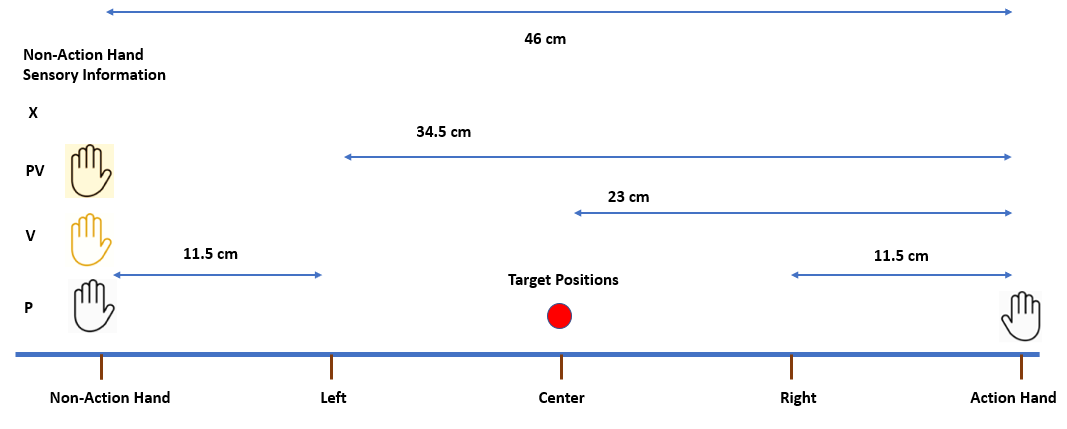
\includegraphics[width=\textwidth, keepaspectratio]{Images/exp1_task.png}
    \caption{Experimental Setup}
    \label{fig:exp1-task}
\end{figure}

\subsection{Calibration} 

At the beginning of the experiment, the participants were given oral instructions to calibrate for spatially aligning the virtual table with the physical table. Five block dots, aligned on x axis, appeared on the table with a distance of 11.5cm between them. The participant rested their right index finger on the right dock. Only the virtual hands were visible during the calibration process, whereas the physical docks were not visible in the virtual environment. Using the arrow keys on the keyboard, the participant was asked to move the rightmost black dot, such that the dot lies under their right index finger. Then, the table height was adjusted by the participant using the keypad enter and plus keys, such that the hand resting on the physical table also appeared to rest on the virtual table. The participant was then asked to rest their left index finger on the left dock, sequentially make contact with the three center dots with their right hand, and then rest the right hand on the right dock, during which the experimenter calibrated the positions of the hand at these five locations respectively.


\subsection{Procedure}


\begin{table}[t]
\centering
\resizebox{\textwidth}{!}{
\begin{tabular}{llll}
\hline 
Block & Action hand Visibility & Non-Action hand Position & Non-Action hand Visibility\tabularnewline
\hline 
Training & Visible & Lap & -\tabularnewline
Feedback & Invisible & Lap & -\tabularnewline
X & Invisible & Lap & -\tabularnewline
P & Invisible & Left dock & Invisible\tabularnewline
V & Invisible & Lap & Visible (Model hand rendered)\tabularnewline
PV & Invisible & Left dock & Visible\tabularnewline
\hline
\end{tabular}}
\caption{Experiment Block structure}
\label{table:block_structure}
\end{table}




The experiment was divided into 6 blocks. Depending upon the block, the participant was instructed regarding the placement of the left hand - either with the left index finger resting on the left dock, or the left hand resting on the participants lap. Furthermore, depending upon the block of the experiment, the left and the right hand were rendered visible or invisible.  

The participants initiated each trial by bringing their right index finger on the right dock. After an audio cue, the target is presented in one of the three target positions. On presentation of the visual target, the participant attempted to make contact with the visual target by making unspeeded reaching action with their right hand towards the target. On contact with the table, the target disappears, indicating the completion of the trial. After completion of the trial, the participant returns the right hand back to the right dock to initiate the next trial.  

The first block of the experiment was the training phase, intended to acquaint the participant with the task and the virtual environment. In the training block, the right hand was rendered visible, while the left hand was placed on the participants lap. The next block was the Feedback block, in which the right hand was rendered invisible. After the participant indicated the position of the target by making contact with the table, a green dot appeared to indicate the location where the participant had made the contact with the table. This served as feedback for the participant, to compare their responses to the actual location of the target.

In the next four blocks, the right hand was rendered invisible as a methodological constraint to introduce uncertainty in the reaching action. The presence and absence of proprioceptive and visual information of the left hand served as experimental manipulations. Proprioceptive information of the the non-action hand was manipulated by asking the participant to rest their left hand on the left dock (Proprioceptive Information present condition) or to rest their left hand on their lap (Proprioceptive Information absent Condition). The Visual information of the non-action hand was manipulated by rendering it visible (Visual Information Present Condition) or invisible (Visual Information Absent Condition). See Table \ref{table:block_structure} for a comprehensive overview of the block design.


For all participants, the first and the second block were Training and Feedback respectively. The order of the remaining four blocks was counterbalanced across participants using the Latin Square Balancing Design. The three target positions were randomized within each block. All six blocks consisted of 60 trials each, with 20 trials for each of the 3 target positions within each block. The participant thus completed a total of 360 trials across six blocks.

\subsection{Experimental Design}
\begin{table}[t]
\centering
\begin{tabular}{rlrrrrlr}
  \hline
 & Effect & DFn & DFd & F & p & p$<$.05 & pes \\ 
  \hline
1 & block & 3.00 & 60.00 & 3.482 & 0.021 & * & 0.148 \\ 
  2 & target\_pos & 1.14 & 22.89 & 10.013 & 0.003 & * & 0.334 \\ 
  3 & block:target\_pos & 3.62 & 72.38 & 1.435 & 0.235 &  & 0.067 \\ 
   \hline
\end{tabular}
\caption{Repeated measures ANOVA results with Greenhouse-Geisser Sphericity Corrections: Reach error $\sim$ Target Position * Visuo-Proprioceptive Information + (1 $\mid$ subject)}
\label{table:rm-anova}
\end{table}

The experiment was set up in a within-subject 4 x 3 factorial design, with two independent variables - Non-Action Hand Information and Target Position. Accuracy in target location estimation was operationalized as \textit{reach error}, which was computed by subtracting the actual target location from the estimated target location indicated by the participants response for each trial. Positive reach error indicates that the estimated target location was an underestimation towards the direction of the action hand, while negative reach error indicates that the estimated target location was an overestimation towards the direction of the non-action hand. Data was analyzed for the four blocks where Non-Action hand information was manipulated (X, P, V, PV). The experiment thus consisted of 12 conditions- 4 (Non-Action Hand Information conditions) x 3 (Target Position conditions). Subject-wise mean reach error was calculated for each of the 12 conditions by computing the average of mean error across trials for each condition, which served as the dependent variable.  

The Outlier criteria was determined as any participant whose any of the mean reach error values fall above Q3 + 3 x IQR or below Q1 - 3 x IQR (Q3 = Third quartile, IQR = interquartile range). On the basis of this criteria, data from one participant was excluded from the analysis.



\section{Results}

\begin{figure}
\centering       
    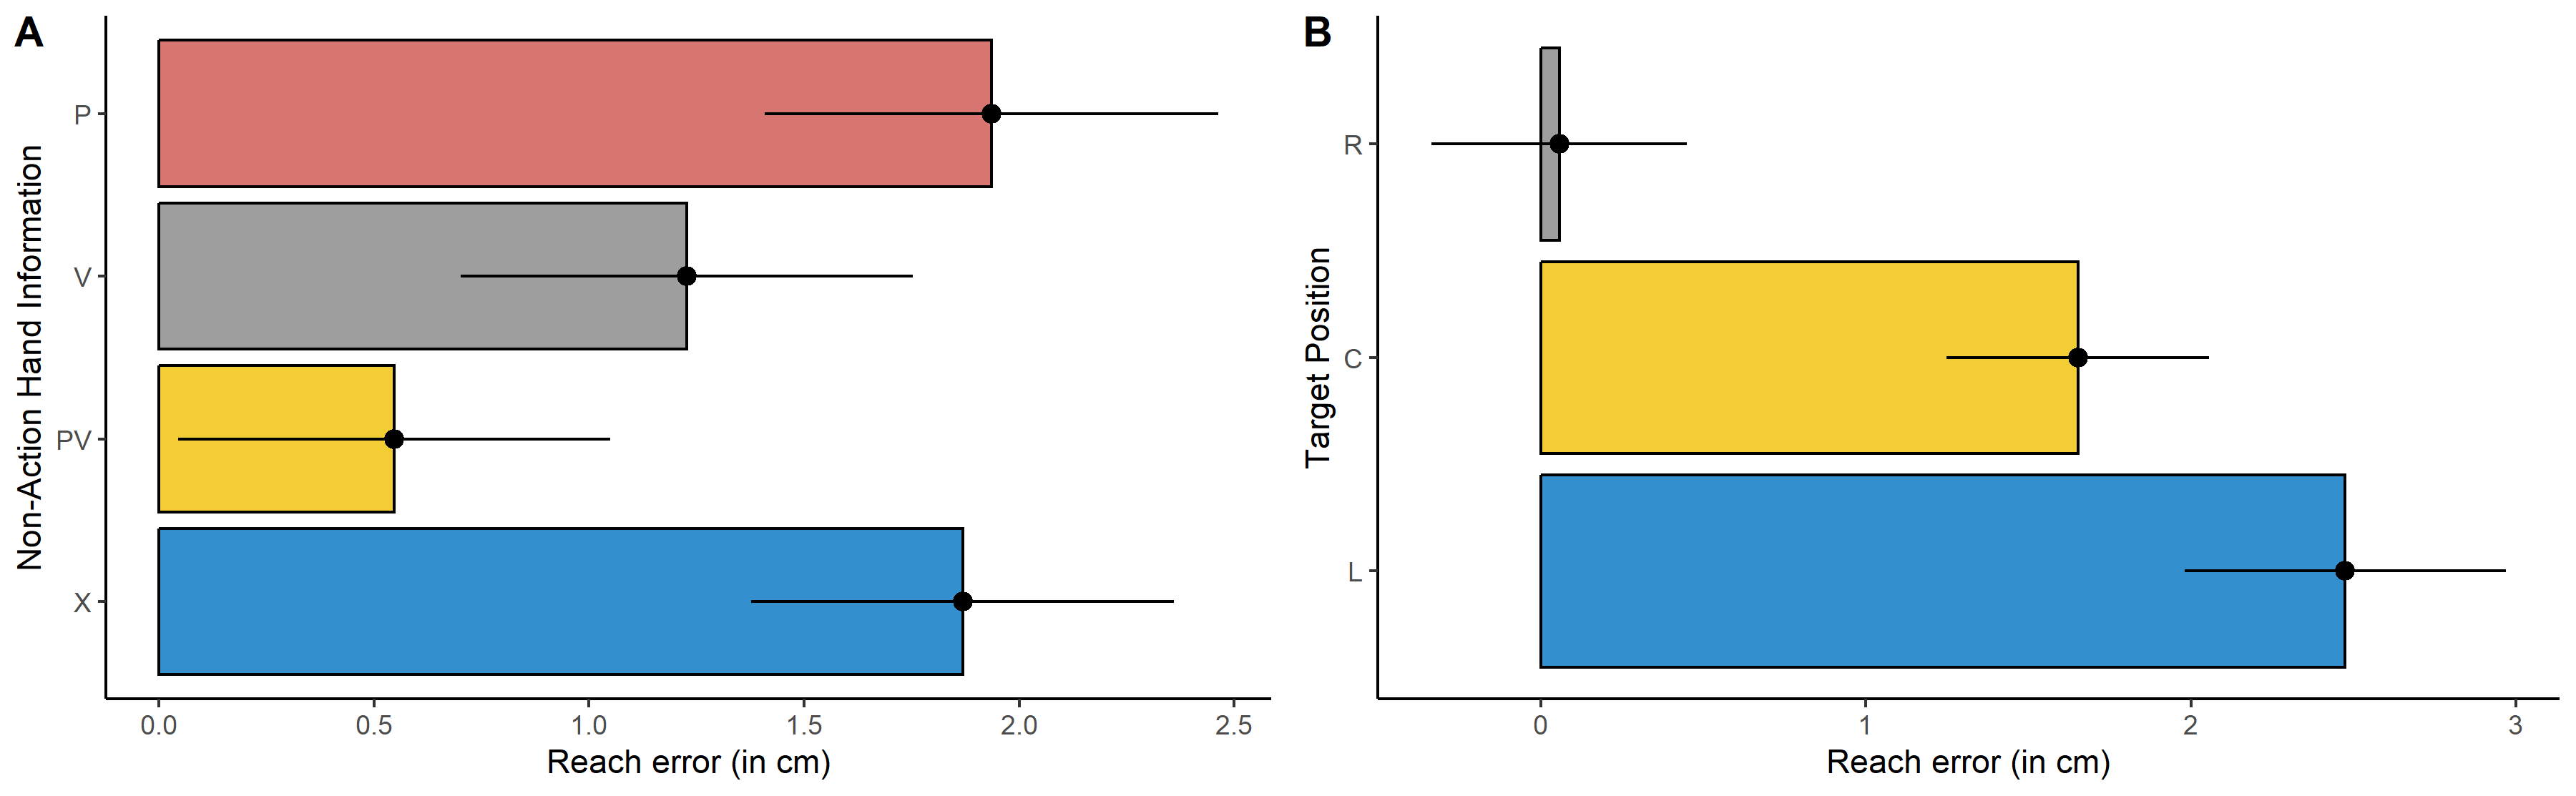
\includegraphics[width=\textwidth, keepaspectratio]{Images/exp1-mre.png}
    \caption{Effect of Non-Action hand information and Target Position on Reach error. The positive values of reach error indicate that the end point of the reach was in the direction of the action hand to the right of the target. The error bars indicate standard error of the mean.}
    \label{fig:exp1-mre}
\end{figure}


A 4 (Non-Action Hand Information: X, V, P, PV) X 3 (Target Position: Left, Center, Right) repeated measures ANOVA was performed to evaluate the effect of the two factors on magnitude of reach error. The analysis demonstrated a significant main effect of both Non-Action Hand Visibility ($F(3,60) = 3.482 , p = 0.021, \eta_{p}^{2} = 0.148$) and Target Position ($F(1.14,22.89) = 10.013, p = 0.003, \eta_{p}^{2} = 0.334$)  (See Table \ref{table:rm-anova}). No significant interaction effect between the two factors was present($F(3.62,72.38) = 1.435, p = 0.235, \eta_{p}^{2} = 0.067$). 

%Post-hoc pair-wise comparisons for analyzing the differences in the reach error between each of the four Non-Action Hand Information condition, using Bonferroni corrected paired t-test, showed that the magnitude of reach error for X and PV conditions differed significantly ($t(20) = 2.9427216, p = 0.048, d = 0.642$). Pair-wise comparisons for analyzing differences in reach error between the three target position conditions showed that reach error magnitude differed significantly between Left and Right positions ($t(20) = 3.223430, p = 0.013, d = 0.703$), and also between Center and Right positions ($t(20) = 3.728681, p = 0.004, d = 0.813$).

Post-hoc pair-wise comparisons for analyzing the differences in the reach error between each of the four Non-Action Hand Information condition, using Holm-Bonferroni corrected paired t-test, showed that the magnitude of reach error for X and PV conditions differed significantly ($t(20) = 2.9427216, p = 0.048, d = 0.642$). Pair-wise comparisons for analyzing differences in reach error between the three target position conditions showed that reach error magnitude differed significantly between Left and Right positions ($t(20) = 3.223430, p = 0.009, d = 0.703$), and also between Center and Right positions ($t(20) = 3.728681, p = 0.004, d = 0.813$).


The results of the experiment show that across all conditions, on average, there is an underestimation in the responses to the estimation of spatial location of the target, that is, the estimated target location is in the direction of the action hand relative to the actual target location. Furthermore, the subjects are more accurate (lower reach error magnitude) when both proprioceptive and visual information of the non-action hand is present (PV condition), as compared to condition in which both proprioceptive and visual information of the non-action hand is absent (X Condition). Moreover, the subjects are most accurate in the Right Target Position, lesser accurate in the Center Target Position, and least accurate in the Left Target Position. 

\section{Discussion}

%The results of this experiment suggest that subjects are more accurate in target location estimation when both visual and proprioceptive information of the hand is provided, even though the hand is reach action task irrelevant.  This result provides support to our conjecture that even task irrelevant body part in proximity to the target affects the representation of the spatial information of the target, suggesting that the target of reach action is represented in an ego-centric frame of reference with respect to the part of body near it. Furthermore, the accuracy of estimating target location is not significantly improved when just uni-sensory information of the non-action hand is present. This suggests that atleast some level of integration between visual and proprioceptive sensory signals of the hand may be necessary for the ego-centric representation of target to occur efficiently. 



The results of the experiment show that the response of the reach action is affected by the position of the target, and the sensory information of the non-action body part which is proximal to the target. The position of the target can be interpreted in two ways- as the distance to be covered by the action hand during the unfolding of action, or as the proximity to the non-action hand. Since there is no interaction effect present between the non-action hand information and the target position, the target position may be interpreted as the distance between the action hand and the target. The decrease in accuracy as the distance between the target position and initial position of action hand suggests that as the distance covered in the reach increases, the greater underestimation is observed in situations of uncertainty, which in this case is the invisibility of action hand.

Regarding the effect of non-action hand information, subjects are more accurate in target location estimation when both visual and proprioceptive information of the non-effector hand is provided, even when the body-part parameters of this hand are not seemingly relevant. This result provides support to our conjecture that even task irrelevant body part in proximity to the target affects the representation of the spatial information of the target, suggesting that the target of reach action is represented in an ego-centric frame of reference with respect to the part of body near it. Furthermore, the accuracy of estimating target location is not significantly improved when just uni-sensory information of the non-action hand is present. This suggests that atleast some level of integration between visual and proprioceptive sensory signals of the hand may be necessary for the ego-centric representation of target to occur efficiently.

However, if the spatial encoding of the the target is indeed anchored to the sensory information which specifies the position of the body-part proximal to the target, the expectation is that the proximity to the target should increase the accuracy of the spatial representation of the target. However, the results indicate the opposite. Thus overall, this suggests that there are two processes which additively influence the spatial encoding of the target- i) underestimation when the reaches are over longer distances, and ii) biasing the target position towards the non-action hand (thus increasing the accuracy) when the target's spatial information is anchored to it when its multi-sensory information is present.



%What exactly does ego-centric anchoring achieve? One possibility is that the anchoring causes a reduced uncertainty regarding the target position, which is indicated by main effect of condition with more accurate action when both proprioceptive and visual information regarding non-target hand was present. However, the lack of increase in accuracy when the target is closer to the non-action hand suggests that there is an interaction between the two processes of i) underestimation when the reaches are over longer distances, and ii) Biasing the target position towards non-action hand when the target representation is anchored to it.






